%%%%%%%% ICML 2021 EXAMPLE LATEX SUBMISSION FILE %%%%%%%%%%%%%%%%%

\documentclass{article}

% Recommended, but optional, packages for figures and better typesetting:
\usepackage{microtype}
\usepackage{graphicx}
\usepackage{subfigure}
\usepackage{booktabs} % for professional tables
\usepackage{multirow}
% hyperref makes hyperlinks in the resulting PDF.
% If your build breaks (sometimes temporarily if a hyperlink spans a page)
% please comment out the following usepackage line and replace
% \usepackage{icml2021} with \usepackage[nohyperref]{icml2021} above.
\usepackage{hyperref}

% Attempt to make hyperref and algorithmic work together better:
\newcommand{\theHalgorithm}{\arabic{algorithm}}

% Define the subsubsubsection command
\newcommand{\subsubsubsection}[1]{%
  \paragraph{#1}\mbox{}\\}





\usepackage[accepted]{icml2021}

\icmltitlerunning{Wine Quality Prediction}

\begin{document}

\twocolumn[
\icmltitle{Wine Quality Prediction}

\begin{icmlauthorlist}
\icmlauthor{Stijn de Preter (852726504)}{ou}
\icmlauthor{Arjan Broer (850166428)}{ou}
\end{icmlauthorlist}

\icmlaffiliation{ou}{Open Universiteit}
\icmlcorrespondingauthor{}{}

% You may provide any keywords that you
% find helpful for describing your paper; these are used to populate
% the "keywords" metadata in the PDF but will not be shown in the document
\icmlkeywords{wine quality, machine learning, neural networks, ANN, SVR }

\vskip 0.3in
]

\section{Brief Introduction}
The assignment is based on the article \cite{dahal2021prediction} and focuses on the reproduction of the article results.
The reproduct is limited to only the Support Vector Regression (SVR) and Artificial Neural Network (ANN) models.
The Ridge Regression (RR) and Gradient Boosting Regression models are not discussed in this report.
The goal of the assignment is to predict the quality of wine based on its physical and chemical properties and understand the methods used to generate the predictions.
The dataset will be analyzed to find the features that most influence the quality of wine and suggestions are provided to improve the hyperparameters of the model for best results.

The research questions discussed in this report are:
\begin{enumerate}
    \item Reproduce the results of the article \cite{dahal2021prediction} using the same dataset and models.
    \item Analyze the dataset to find the features that most influence the quality of wine.
    \item Provide suggestions to improve the hyperparameters of the model for best results.
\end{enumerate}

\section{Methods}
The methods used for this assignment are based on the article \cite{dahal2021prediction} and include Support Vector Regression (SVR) and Artificial Neural Network (ANN) models.
The impact of the features is analyzed using SHAP (SHapley Additive exPlanations) values and the Pearson correlation coefficient. Improvements on the both the SVR and ANN models are investigated and reported.

\subsection{Reproduce the results}
In order to compare the results of the article with our results, a visualization was made. The values of the article \cite{dahal2021prediction} are compared with our results repeatedly. Our results are reproduced repeatedly with different test and training data each time. This way we are sure that it is not a lucky shot but we get a realistic picture of how our models perform.
Also, standardization has been applied to the data features of the dataset so not to the quality column.

\subsection{Impact of the features}
The article analyses the impact of individual features on the quality of the wine.
This analysis is done by looking at the correlation between the features and the quality of the wine.
The correlation is calculated in the article using the Pearson correlation coefficient.
The Pearson correlation coefficient is a measure of the linear correlation between two variables.

By using SHAP (SHapley Additive exPlanations) values, the impact of the features on the model can be analyzed in more detail.
The explanation of the model should reflect a similar result as compared to the pearson correlation coefficient.
Shapley values are created by using the Shapley value method, which is a method from cooperative game theory. Effectively it will calculate the contribution of each feature to the model output by looking at the impact of each feature on the model output.
\cite{lundberg2017unified} describes in detail how the impact of individual features is determined by retraining the model with this a feature excluded.
Then the impact of the feature on the model output is calculated by looking at the difference between the model output with and without the feature.
Diagrams used here to explain the impact of features are the summary plot and dependency plot.
The summary plot shows the impact of all features on the model output ordered from strongest impact to weaker impact.
The dependency plot shows the impact of a single feature on the model output.

\subsection{Improve the model}
For optimizing the hyperparameters, BayesSearch is used for SVR. For ANN, gridsearch was used to examine the impact of the hyperparameters. The optimized models will be evaluated and compared with the values from the article and with the reproduced models.

\section{Experimental Results}
This chapter, experimental results, is split into 3 parts: A short general piece, a piece on SVR and a part on ANN.

\subsection{Datasets}
When exploiting the data it was found that the information given in the article about the data did not match the information about the data. The article indicates that the red wine dataset was used. Based on the number of rows and other metadata (averages, Median, ...) we see that the white wine dataset was used. In the rest of this article we will work with the white wine dataset.

The correlation between all the columns has also been visualized in figure \autoref{fig:correlation-matrix} and investigated. The following findings emerged:
\begin{itemize}
	\item Alcohol has the greatest correlation with quality.
	\item Density and residual sugar are inversely proportional, which can also be explained. Dissolved sugar increases the density.
	\item Density and alcohol have a directly proportional relationship. This can also be explained. Alcohol is lighter than water, more alcohol makes the liquid less dense.
	\item Residual sugar and alcohol are inversely proportional. This can be explained by the fact that the sugar is converted into alcohol. The more residual sugar is left, the less alcohol will have been made.
\end{itemize}

\begin{figure}
	\centering
	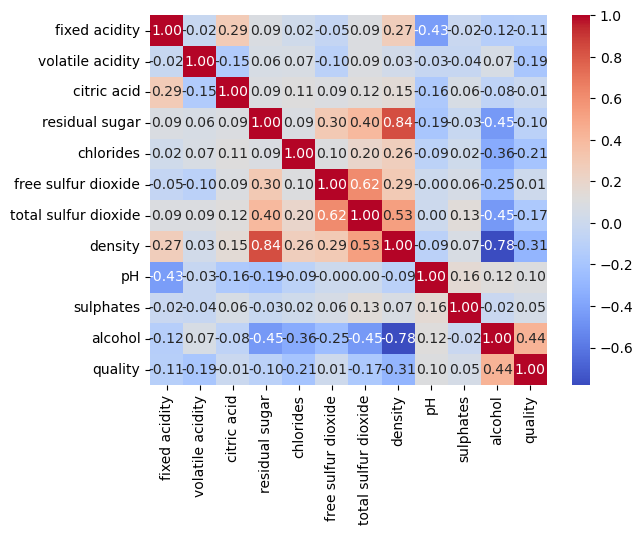
\includegraphics[width=\linewidth]{figures/correlation_matrix.png}
	\caption{Correlation between the columns of the white wine dataset}
	\label{fig:correlation-matrix}
\end{figure}


\subsection{SVR}

\subsubsection{Datasets}
The article indicates that the data is split into training data and testing data with a ratio of 3:1. This is also the ratio of the splits that was applied in further research.

\subsubsection{Implementation Details}

\subsubsubsection{Reproduce the results}
The results of the article are simulated by using the parameters mentioned in the article. The following parameters are mentioned: kernel=rbf, cost = 0.95 and Gamma = 0.13. For all other parameters, the default parameters of sklearn are chosen, except for the Tolerance for stopping criterion, which is set to 0.0001 to obtain the best possible result and because the cost is negligible given the small dataset.
How the training data is chosen is unknown, so the split between training and test data is performed multiple times. In this way, there is a realistic picture of the models that generate these parameters.

\subsubsubsection{Impact of the features}
The trained model used for analyzing the impact of features is the same as the model used for reproducing the results.
When reproducing the results it was shown that the selection of a train and test set has an impact of on the model performance.
The training set split used for the feature analysis results from applying {\texttt{random\_state=1}}.

For the shap explainer the KernelExplainer was used.
The KernelExplainer is a model-agnostic explainer that can be used to explain the output of any machine learning model.
As background data a random sample of 200 rows from the training data was used.
The KernelExplainer uses the background data to estimate the expected value of the model output.
The KernelExplainer is a computationally expensive method, so a smaller sample size is used for the background data.
Then a random sample of 50 rows as test data has been taken from the test data to explain the model output.
The SHAP values are calculated for these 50 test samples.
For higher accuracy both the background data and test samples can be increased, but this will increase the computation time.
Having only a home laptop available, the sample size is kept small to keep the computation time reasonable.

Both the summary plot and the dependency plot are used to visualize the impact of the features on the model output.
These plots are both generated using the same SHAP values calculated for the test samples.

\subsubsubsection{Improve the model}
To optimize the model, the cost and gamma were examined. BayesSearch was used to find a model with the lowest possible mean squared error. The result is visualized in a scatter plot where green points indicate a good model and red points indicate a less good model.
The new parameters will be used to train a model 100 times. Each time with different train and test data, but the ratio (3:1) will be maintained. These 100 trained models will be visually compared with the article \cite{dahal2021prediction} model.

\subsubsection{Results}

\subsubsubsection{Reproduce the results}

The results are visualized in \autoref{fig:Reproduce-SVR-the-results}. The important part is how the results are compared to the test data. The correlation and the MAPE give better results than the article \cite{dahal2021prediction}. While the MSE of the reproduced model are slightly worse.

\begin{figure}
\centering
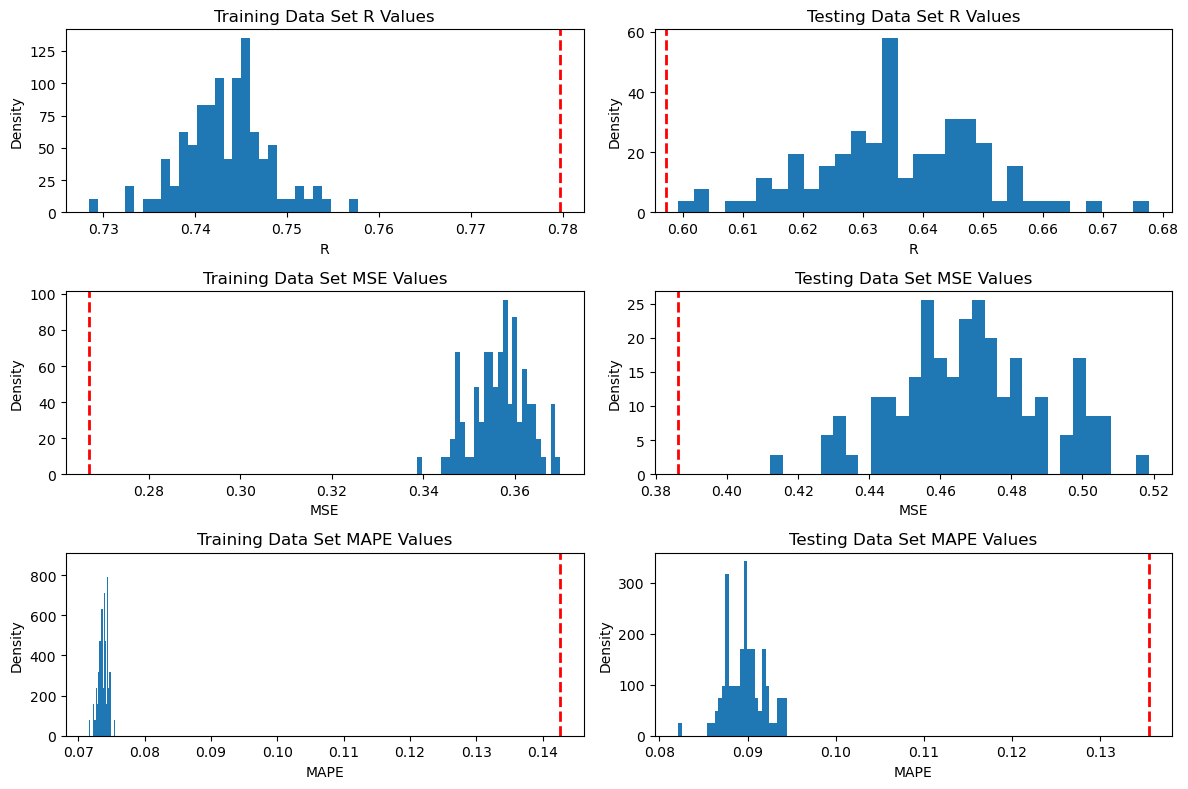
\includegraphics[width=\linewidth]{figures/SVR_reproduce_the_results.png}
\caption{Comparison between the SVR model from the article (red dashed line) and the reproduced model (blue bars)}
\label{fig:Reproduce-SVR-the-results}
\end{figure}

\subsubsubsection{Impact of the features}
In \autoref{fig:summary-plot-svr} \nameref{fig:summary-plot-svr} the impact of all features is visualized.
From this diagram it is clear that Alcohol has the most positive impact on the model output.
The blue values indicate a low value of the feature and the red values indicate a high value of the feature.
The impact on the model output is shown on the x-axis. For alcohol the blue values are on the left side of the plot and the red values are on the right side of the plot, meaning the impact is positive.
Residual sugar has a same positive impact on the model output, but the impact is slightly smaller than for alcohol.
density and volatile acidity have a negative impact on the model output. The blue values are on the right side of the plot and the red values are on the left side of the plot, meaning the impact is negative.
The features with a very weak correlation to the output are: chlorides, free sulfur dioxide and total sulfur dioxide. The impact of these features is very small compared to the other features.
The SHAP values for those features are more chaotic and do not show a clear trend.

In figure \autoref{fig:dependency-plot-svr} \nameref{fig:dependency-plot-svr} the impact of the individual features are visualized.
The dependency plot shows the impact of each feature on the model output.
The color of the dots indicates the value \textbf{(=impact?)} of the feature, with red indicating a high value and blue indicating a low value.
The y-axis shows the impact of the feature on the model output.

The plot for alcohol shows that the impact of alcohol on the model output is positive.
This means that a higher value of alcohol leads to a higher quality of wine.
The trend of the values is clearly visible in the plot, showing a positive correlation between the feature and the model output. %naam plot toevoegen
This is also confirmed by the Pearson correlation coefficient, which shows a positive correlation between alcohol and quality.

The plot for density show that the impact of density on the model output is negative.
This means that a higher value of density leads to a lower quality of wine.
just as with alcohol, the trend of the values is clearly visible in the plot, showing a strong negative correlation between the feature and the model output.

The plot for chlorides shows that the impact of chlorides on the model output is also negative. Again this corresponds with the Pearson correlation coefficient, which shows a negative correlation between chlorides and quality.

The feature with the least impact on the model output is Free sulfur dioxide.
The plot shows that the impact of Free sulfur dioxide on the model output is positive.
This means that a higher value of Free sulfur dioxide leads to a higher quality of wine.
However, the trend of the values is not clearly visible in the plot, showing a weak correlation between the feature and the model output.
This is also confirmed by the Pearson correlation coefficient, which shows a weak positive correlation between Free sulfur dioxide and quality.
Notable is that Free sulfur dioxide has a strong positive trend for the lower values. This suggests that the feature has a minimum value for the quality of wine.
This was not visible in the pearson correlation coefficient because the correlation coefficient is calculated over the entire dataset.

\begin{figure}
	\centering
	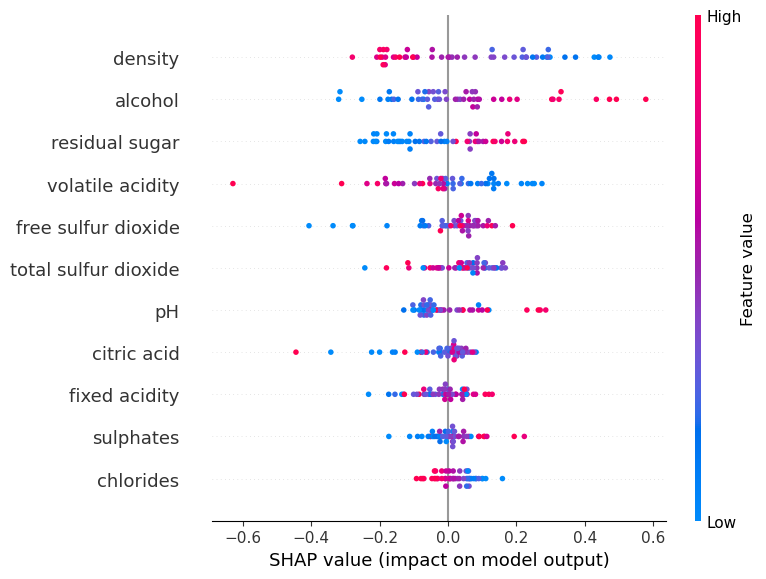
\includegraphics[width=\linewidth]{figures/shap-summary-svr.png}
	\caption{Summary plot of the features for SVR}
	\label{fig:summary-plot-svr}
\end{figure}

\begin{figure}
    \centering
    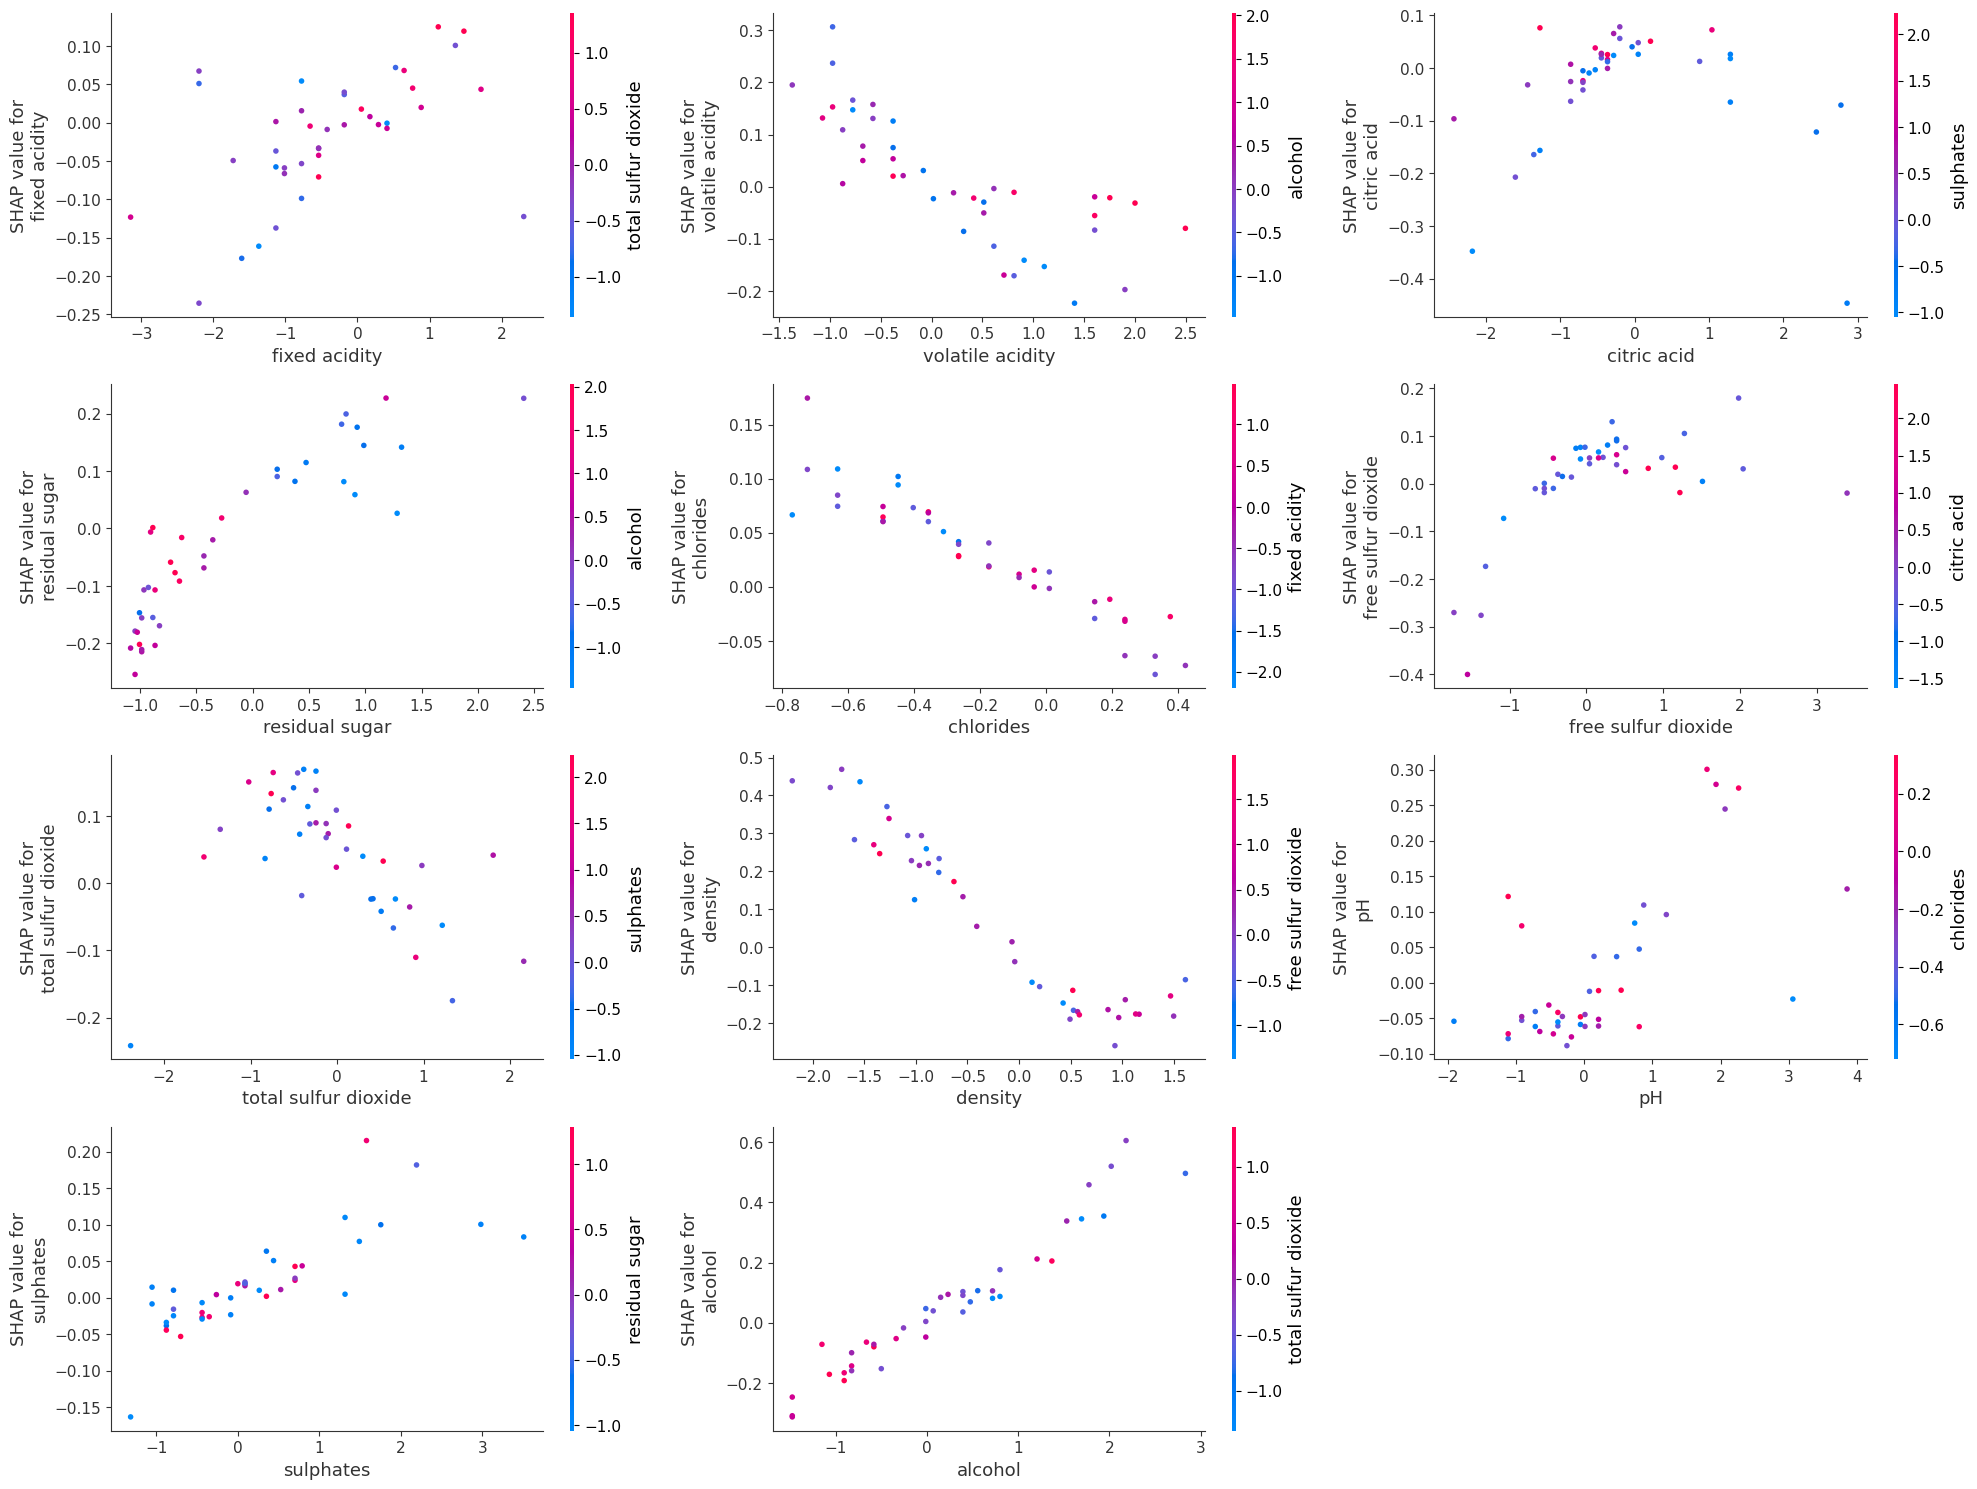
\includegraphics[width=\linewidth]{figures/shap-dependency-svr.png}
    \caption{Dependency plot of the features for SVR}
    \label{fig:dependency-plot-svr}
\end{figure}

\subsubsubsection{Inprove the model}

In \autoref{fig:Bayesian-search-for-optimal-gamma-and-cost} the best possible values for gamma and cost are examined. The non-optimized model (the model with the parameters as indicated in the article \cite{dahal2021prediction} ) is visualized by a blue sphere.
\begin{figure}
    \centering
    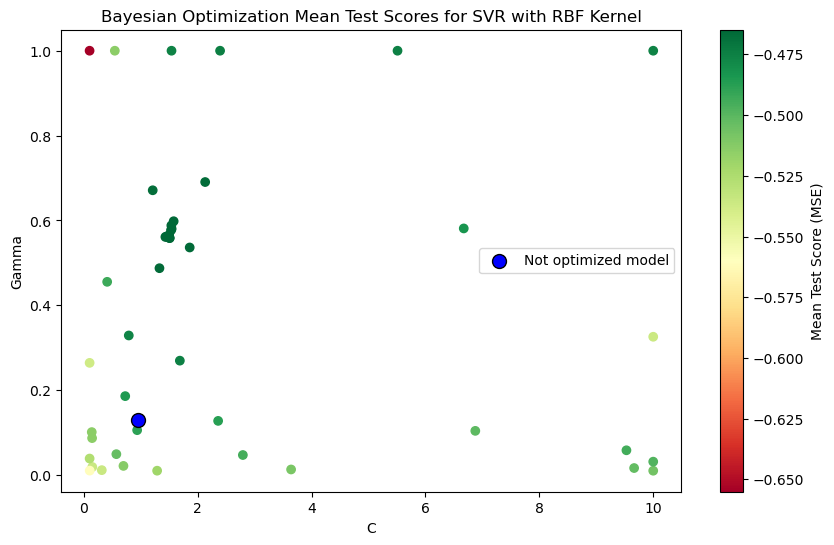
\includegraphics[width=\linewidth]{figures/bayesian_optimization.png}
    \caption{Bayesian search for optimizing gamma and cost. Green indicates better hyperparameters. Blue indicates the parameters from the article.}
    \label{fig:Bayesian-search-for-optimal-gamma-and-cost}
\end{figure}

The most optimal parameters are: cost=1.51 and gamma=0.558.
In \autoref{fig:optimized-SVR-model} we see how the model performs compared to the values of the model of the article \cite{dahal2021prediction} (dashed line) and compared to the non-optimized model (dotted line). 
Based on the three evaluation criteria (correlation, RMSE and MAPE) the model consistently outperforms the non-optimized model. The parameters perform significantly better based on the training data suggesting overfitting, but the results from the testing data are also (slightly) better indicating no overfitting.
\begin{figure}
	\centering
	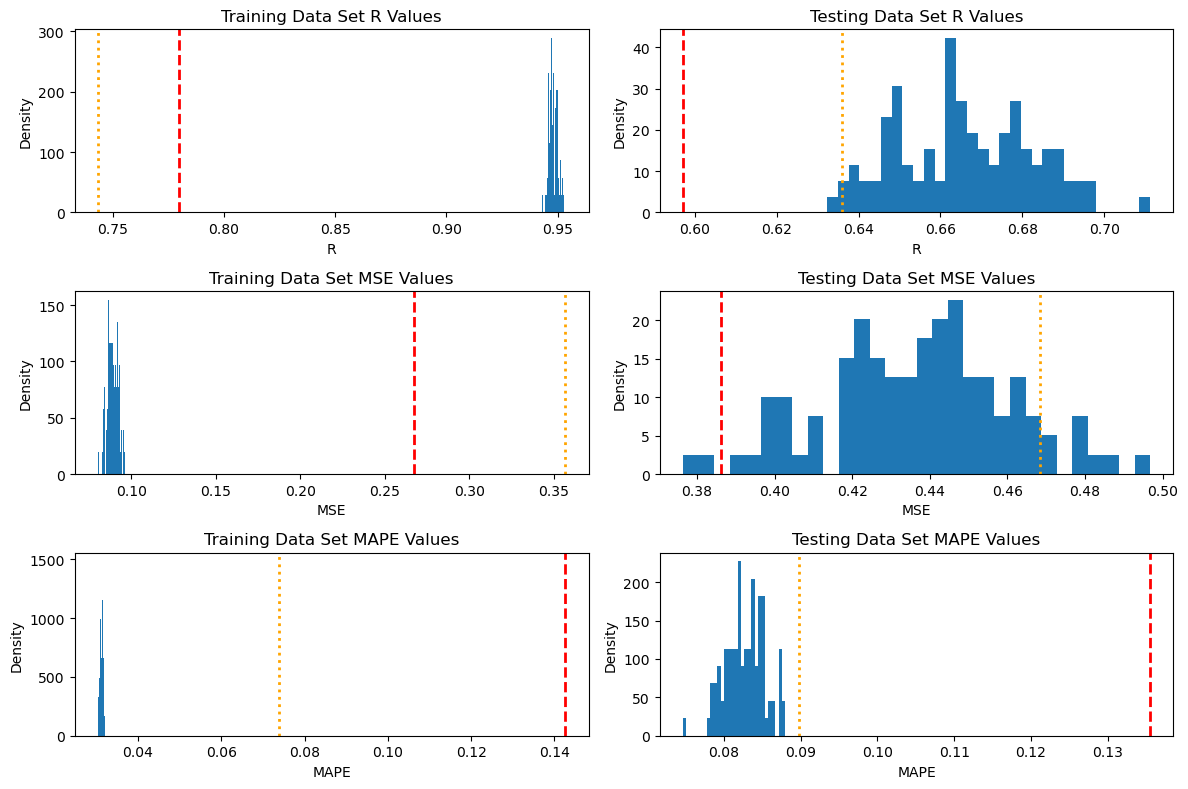
\includegraphics[width=\linewidth]{figures/SVR_optimized_model.png}
	\caption{An optimized SVR model (blue bars) compared to the model from the article (red dashed line) and the reproduced model (orange dotted line)}
	\label{fig:optimized-SVR-model}
\end{figure}


\subsubsection{Discussion}
%Additionally, you can include a separate discussion section in which you summarize the results, indicate possible limitations of your work, and provide suggestions for future research.

The results of the article have been reproduced. The impact of the features has been investigated. And the model has been optimized. All this while the article does not seem reliable because of the incorrect naming of the data set (namely red wine instead of white wine)


\subsection{Citing references}
%%%LaTeX manages the citations for you. You simply have to add the bibtex entry for the reference in the references.bib file and you can use the citation in the paper \cite{langley00}. You can also cite multiple references in one command \cite{DudaHart2nd,Newell81,kearns89}. The bibtex entries for a paper can be obtained in websites such as google scholar or dblp.

\subsection{ANN}

\subsubsection{Datasets}
In the article \cite{dahal2021prediction} it is stated that the train-validation-test ratio is 60-20-20. This ratio has been maintained for reproducing and optimizing the model.

\subsubsection{Implementation Details}

\subsubsubsection{Reproduce the results}
The article \cite{dahal2021prediction} mentions the following parameters: 1 input layer, 3 hidden layers (each with 15 neurons) and one output layer with the Adam optimizer.
As activation function relu was chosen and the mean squared error as loss to optimize. The following parameters were not specified so they were filled in with the following values: number of epochs = 50 and batch size = 16.
How the training data is chosen is also unknown, so the split between training and test data is performed multiple times. In this way, there is a realistic picture of the models that generate these parameters. 

\subsubsubsection{Impact of the features}
The analysis of the impact of the feature is done in the same way as with the SVR model.
We need to be able to compare the results of the feature impact analysis, so the same KernelExplainer is used as with the SVR model.
The KernelExplainer is a model-agnostic explainer that can be used to explain the output of any machine learning model.
In contrast the DeepExplainer is a model-specific explainer that can be used to explain the output of a deep learning model.
The performance of the DeepExplainer is far better compared to the KernelExplainer and seems to have a similar output as the KernelExplainer.
The KernelExplainer is prioritized because it is model-agnostic and as such eliminates differences in result due to different Explainer implementations.



\subsubsubsection{Inprove the model}
In a perfect world, all hyperparameters and all possible models would be tested. However, due to limited time and access to resources, it was decided to look at the number of hidden layers and the number of neurons.
Gridsearch will be used to see if the model can be optimized by adjusting the number of neurons in the hidden layers.
It was also considered to reduce the number of hidden layers to one. The reasoning behind this is that the data is not that complex and that the complexity of the three layers would be unnecessary. With one hidden layer, the impact of the number of neurons is also investigated using Gridsearch. And once an optimum has been found, the impact of batch size and epochs is also examined.

\subsubsection{Results}

\subsubsubsection{Reproduce the results}

In \autoref{fig:ANN-reproduce-the-results} the original model is indicated by a red dashed line. 100 models (with the selected parameters) were trained and shown as blue bar charts. The average of the bar charts is shown by an orange dotted line.
The R values are very similar. The MSE results are worse than those of the model from the article while the MAPE results are better than those from the article.
The combination of a higher MSE and a lower MAPE may indicate that most forecasts are accurate, but there are some exceptions with large errors that increase the MSE.
This must be put into perspective, because we are talking about very small differences compared to the original model. If we know that the quality has no significant figures, the differences compared to the original model are negligible.

\begin{figure}
	\centering
	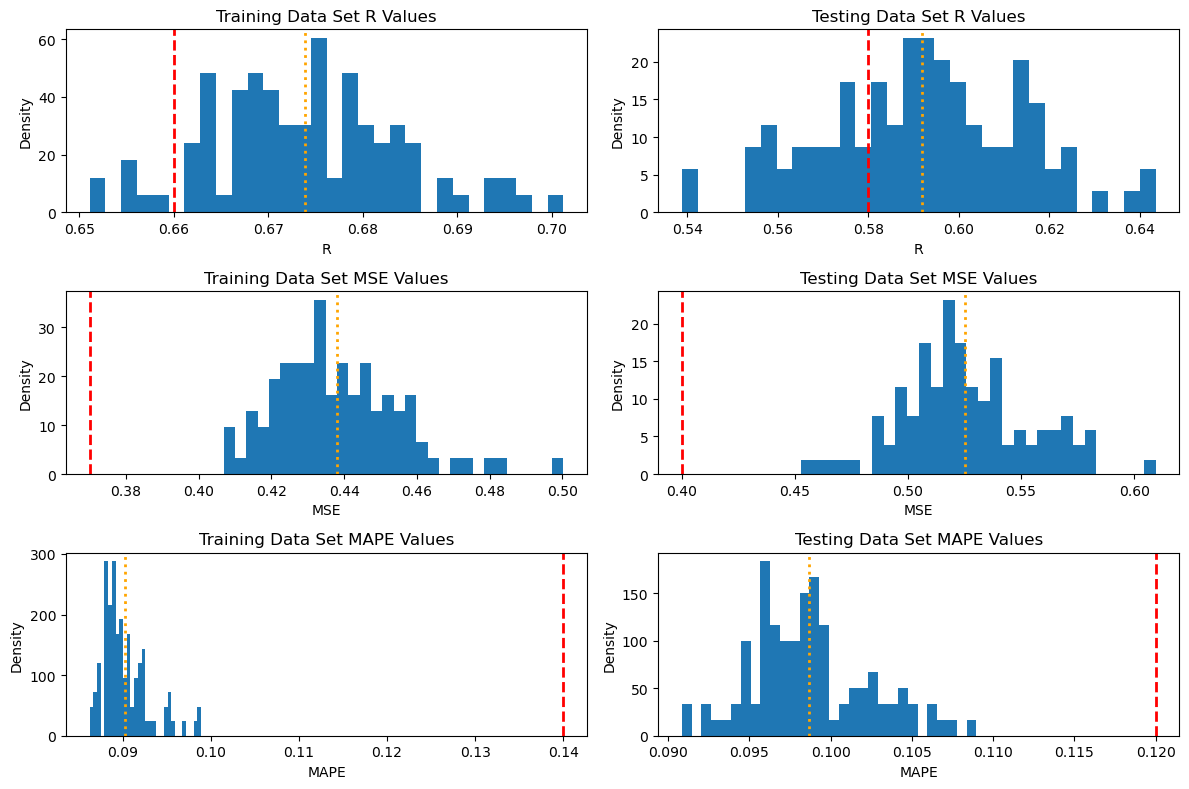
\includegraphics[width=\linewidth]{figures/ANN_reproduce_the_results.png}
	\caption{An reproduced ANN model (blue bars) compared to the model from the article (red dashed line). The average of the reproduced model is also indicated with an orange dotted line.}
	\label{fig:ANN-reproduce-the-results}
\end{figure}


\subsubsubsection{Impact of the features}
The summary plot for the ANN model is shown in figure \autoref{fig:summary-plot-ann} \nameref{fig:summary-plot-ann}.
In this summary plot it is shown that the most important feature is the alcohol as this one is shown on top.
The impact of the alcohol is positive, which means that a higher value of alcohol leads to a higher quality of wine.
Next are residual sugar and density. The impact of residual sugar is positive, while the impact of density is negative.
This is in line with the expectations from the dataset analysis. Residual suger and density are naturally correlated.
Other features can be read in the same way as being positive (blue to red) or negative (red to blue), but are less important than the three features mentioned above.
The features lower in the graph have a very small impact on the model output.
The impact of these features is very small compared to the other features.

\begin{figure}
	\centering
	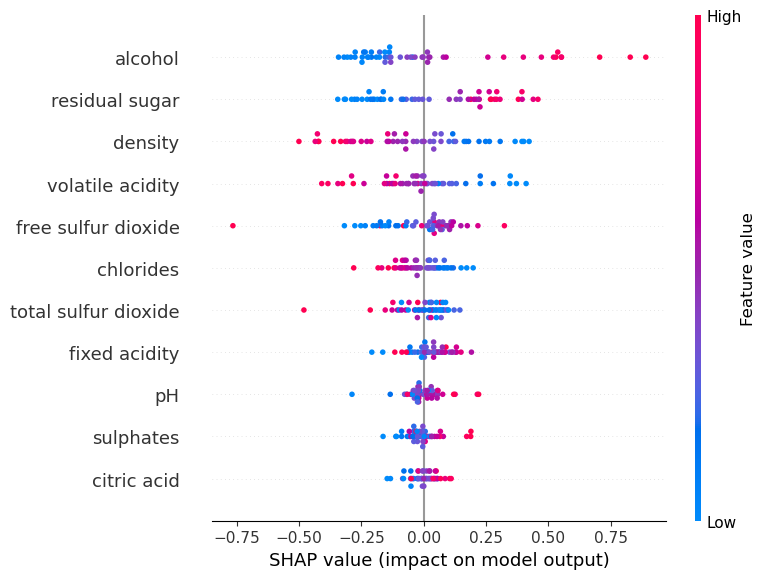
\includegraphics[width=\linewidth]{figures/shap-summary-ann.png}
	\caption{Summary plot of the features for ANN}
	\label{fig:summary-plot-ann}
\end{figure}

Fixed acidity, pH, sulphates and citric acid show more chaotic values and do not show a clear trend.
This can also be seen int the dependency plot in figure \autoref{fig:dependency-plot-ann} \nameref{fig:dependency-plot-ann}.
Where other diagrams how a clear upward or downward trend, the dependency plot for these features shows a more chaotic picture.
This choatic picture results in a low correlation with the model output.

\begin{figure}
	\centering
	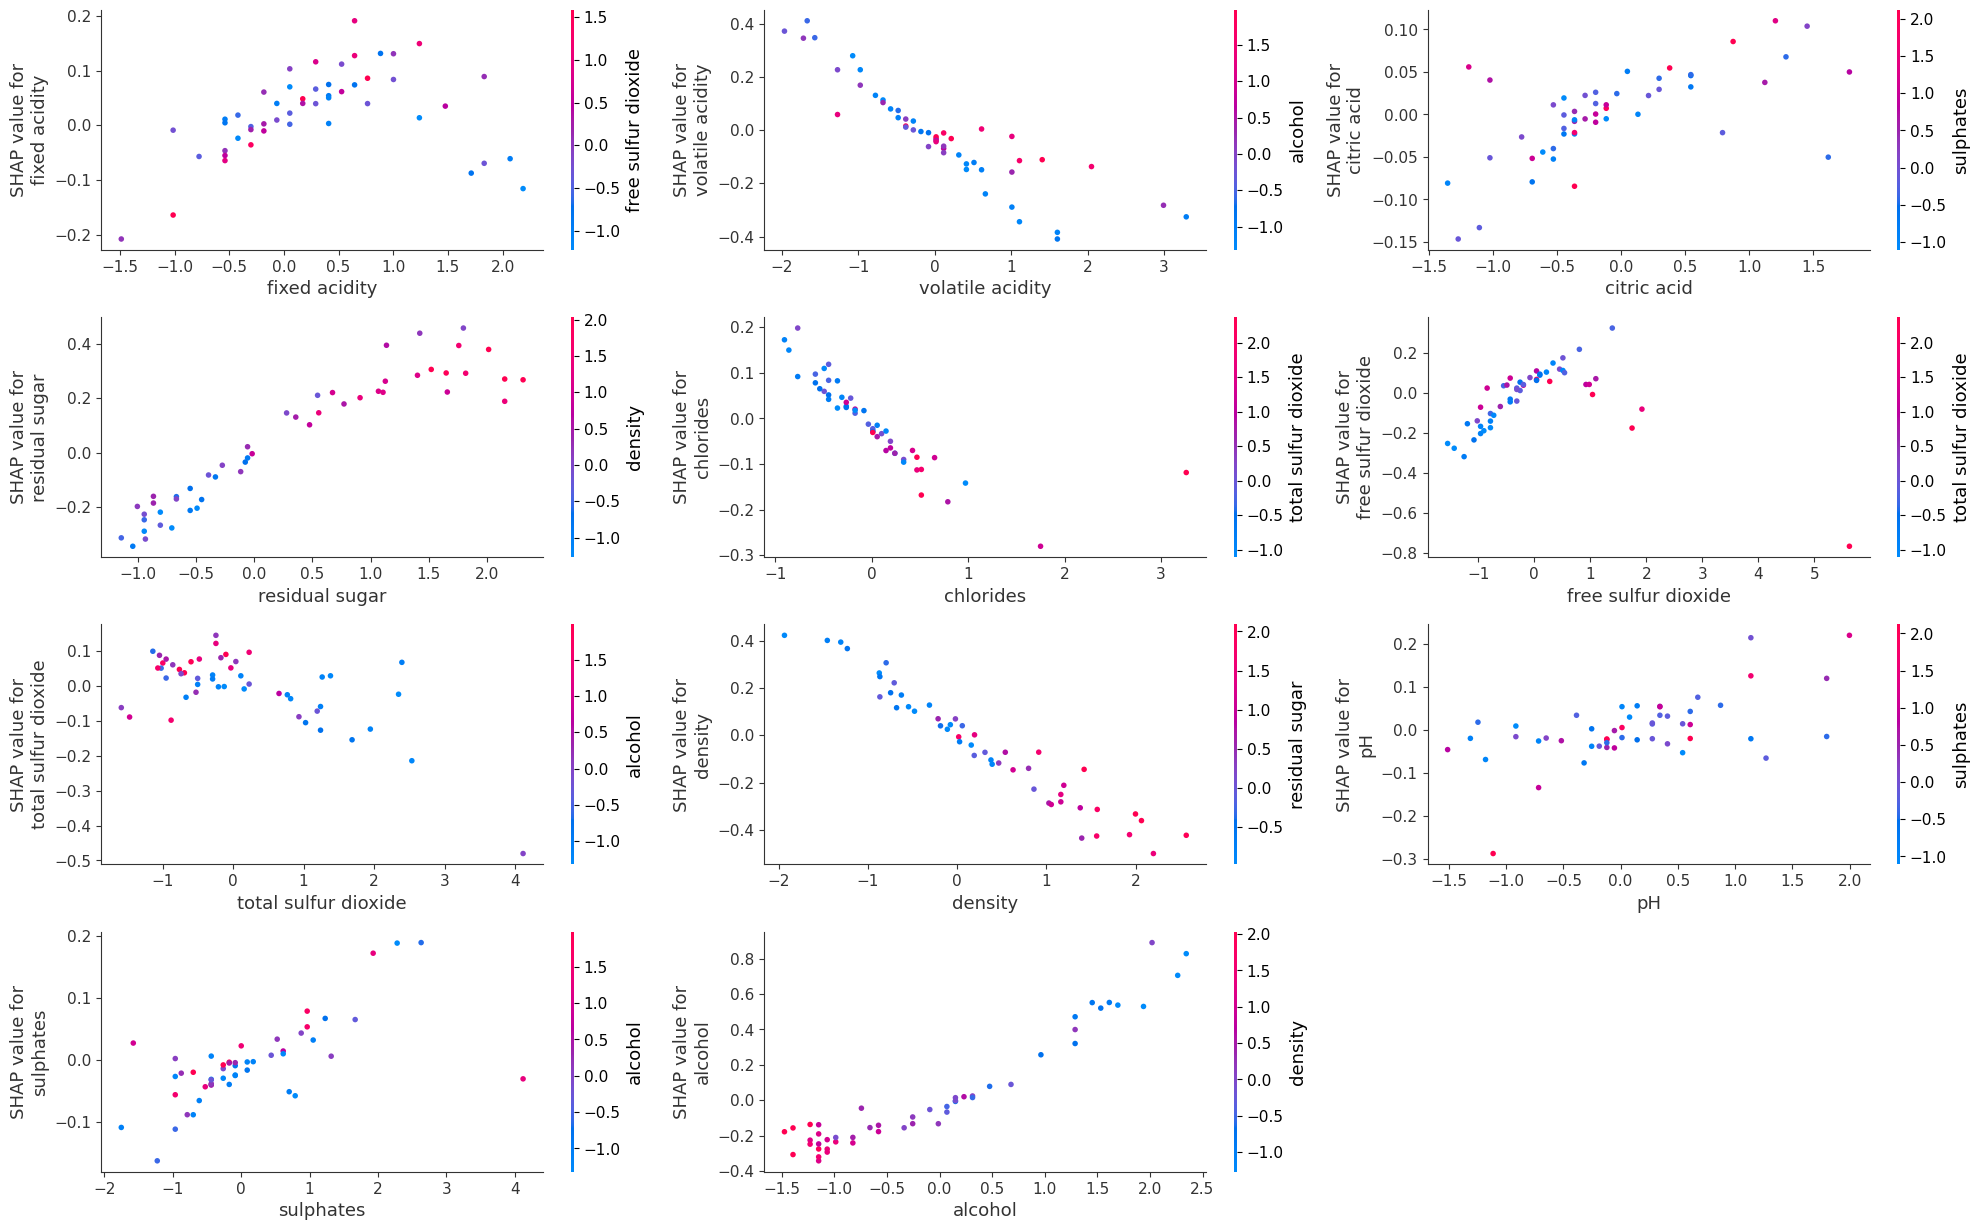
\includegraphics[width=\linewidth]{figures/shap_dependency_ann.png}
	\caption{Dependency plot of the features for ANN}
	\label{fig:dependency-plot-ann}
\end{figure}

\subsubsubsection{Inprove the model}
Based on \autoref{fig:ANN-impact-neurons-3layers} it can be concluded that the model with 15 neurons for each layer is quite well chosen. Increasing the number of neurons will certainly not give better results.

\begin{figure}
	\centering
	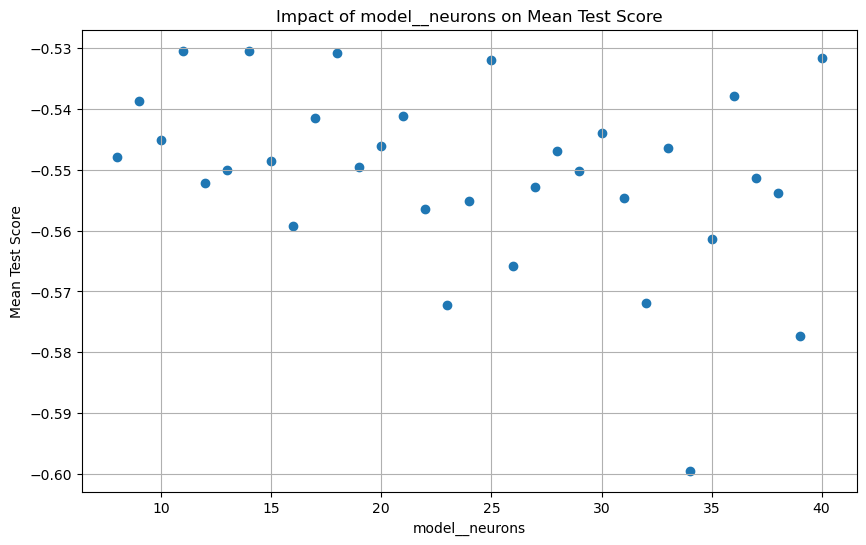
\includegraphics[width=\linewidth]{figures/ANN_impact_neurons_3layers.png}
	\caption{The effect of number of neurons on an ANN model with 3 hidden layers}
	\label{fig:ANN-impact-neurons-3layers}
\end{figure}

With one neuron the story is different, see \autoref{fig:ANN-impact-neurons-1layer}. The model improves as the number of neurons increases with a flattening starting around 70 neurons. With these 70 neurons the impact of batch size and epochs was investigated with the aim of finding a better model.

\begin{figure}
	\centering
	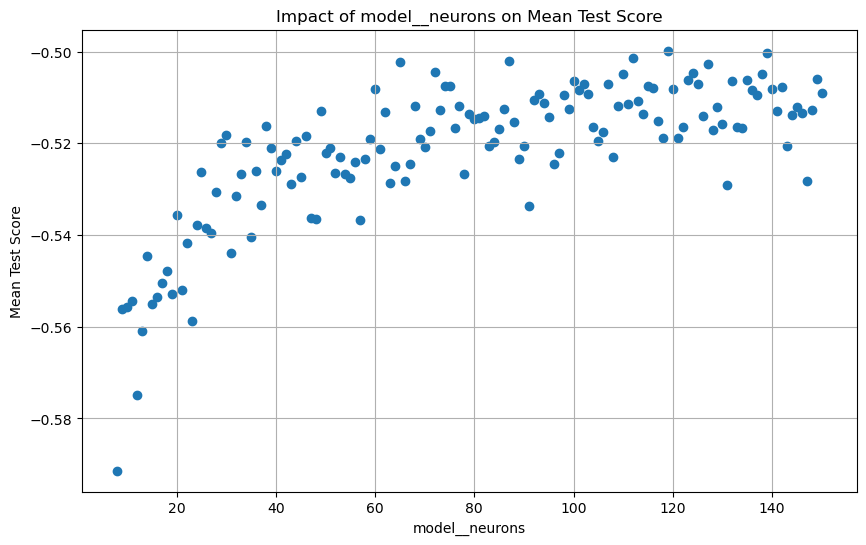
\includegraphics[width=\linewidth]{figures/ANN_impact_neurons_1layer.png}
	\caption{The effect of number of neurons on an ANN model with one hidden layer}
	\label{fig:ANN-impact-neurons-1layer}
\end{figure}

\autoref{fig:ANN-impact-epochs-1layer} and \autoref{fig:ANN-impact-batchsize-1layer} show the results of a grid search for a better model around number of epochs and batch size.
As expected we see that we get better models at higher epochs and smaller batch sizes. For the final model epochs = 40 and batch size = 16 were chosen.


\begin{figure}
	\centering
	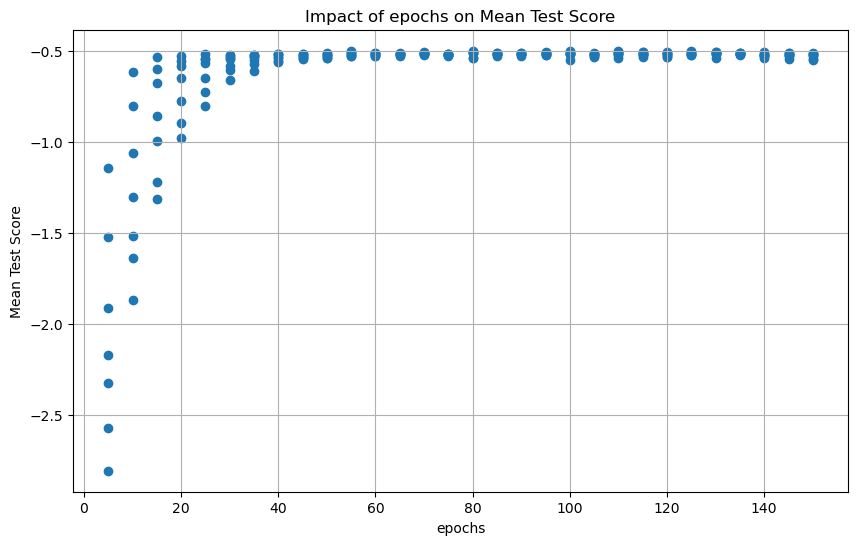
\includegraphics[width=\linewidth]{figures/ANN_impact_epochs_1layer.png}
	\caption{The effect of number of epochs on an ANN model with one hidden layer}
	\label{fig:ANN-impact-epochs-1layer}
\end{figure}

\begin{figure}
	\centering
	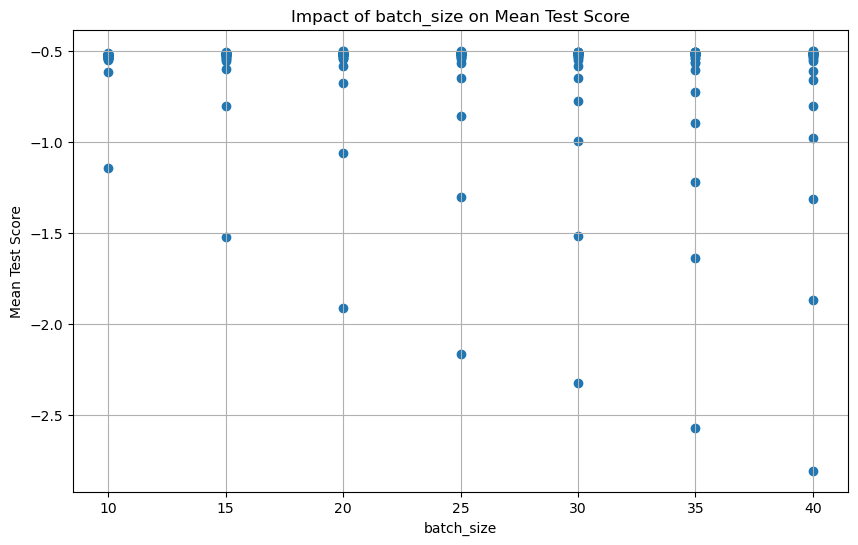
\includegraphics[width=\linewidth]{figures/ANN_impact_batchsize_1layer.png}
	\caption{The effect of number of batch size on an ANN model with one hidden layer}
	\label{fig:ANN-impact-batchsize-1layer}
\end{figure}

\autoref{fig:ANN-optimized-model} shows the model from the article with a red dashed line and the reproduced model with an orange dotted line. The blue bars show an optimized model with one layer (with 70 neurons). Both the R values, MSE and MAPE give better results than the reproduced model. This improvement is only minimal.


\begin{figure}
	\centering
	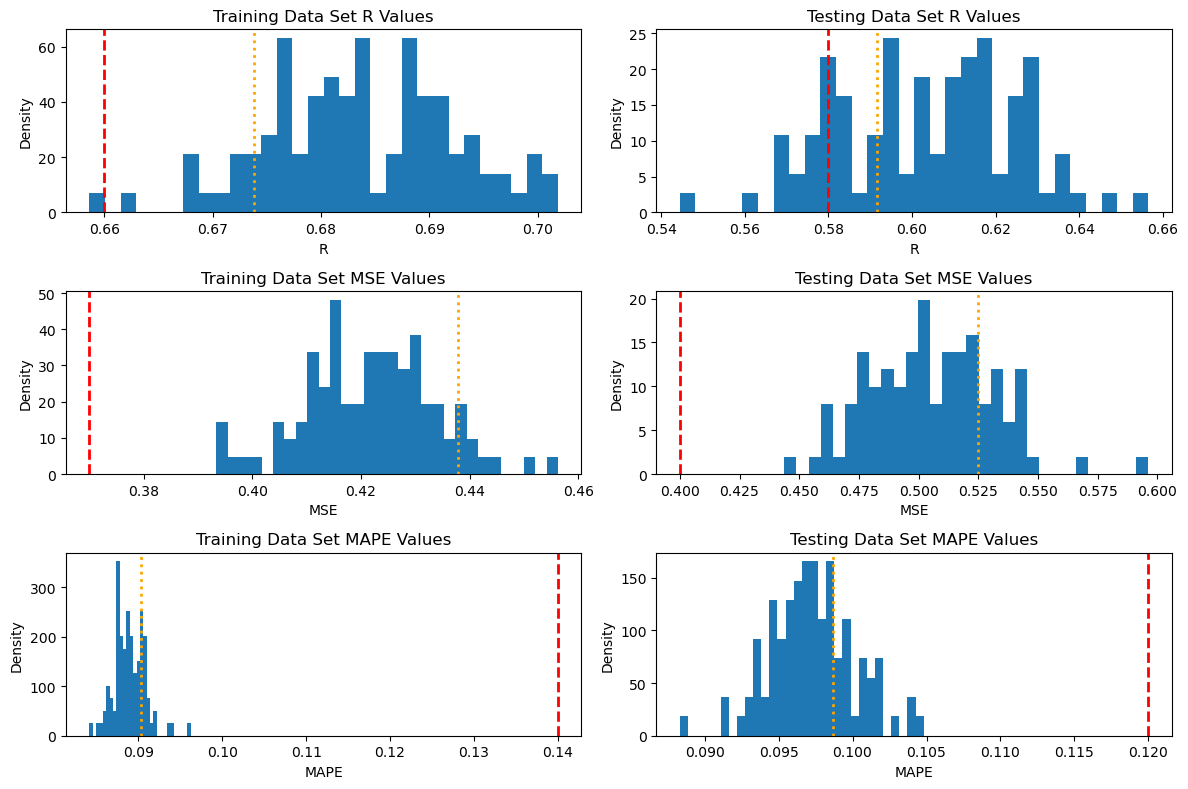
\includegraphics[width=\linewidth]{figures/ANN_optimized_model.png}
	\caption{An optimized ANN model (blue bars) compared to the model from the article (red dashed line) and the reproduced model (orange dotted line)}
	\label{fig:ANN-optimized-model}
\end{figure}




\subsubsection{Discussion}

%nog aan te vullen!


\subsubsection{Citing references}


\bibliography{references}
\bibliographystyle{icml2021}


\end{document}

